\documentclass[border=4pt]{standalone}
\usepackage{amsmath, amssymb, amsfonts}
\usepackage{tikz}
% Shared TikZ style for the deep-learning computation-graph figures.
% Change notation/appearance in ONE place here and rebuild all figures.
\usetikzlibrary{arrows.meta, positioning, calc}

% Colours for forward-pass / backprop highlights
\definecolor{fwdblue}{RGB}{0,0,255}
\definecolor{bpred}{RGB}{255,0,0}

\tikzset{
    % filled dot used for inputs, biases and indicator vectors
    unit/.style={circle, fill=black, inner sep=0pt, minimum size=5pt},
    % linear transformation node (weighted sum), drawn as a circled plus
    sumop/.style={circle, draw, thick, inner sep=1pt, minimum size=16pt},
    % non-linear transformation, a labelled box with vertical text
    opbox/.style={draw, thick, minimum width=22pt, inner sep=6pt},
    % directed edges
    edge/.style={-{Latex[length=6pt]}, thick},
    % edge labels (variable names on the wires)
    wire/.style={font=\normalsize, inner sep=2pt},
}

% vertical text for the operation boxes
\newcommand{\vlabel}[1]{\rotatebox{90}{#1}}


\begin{document}
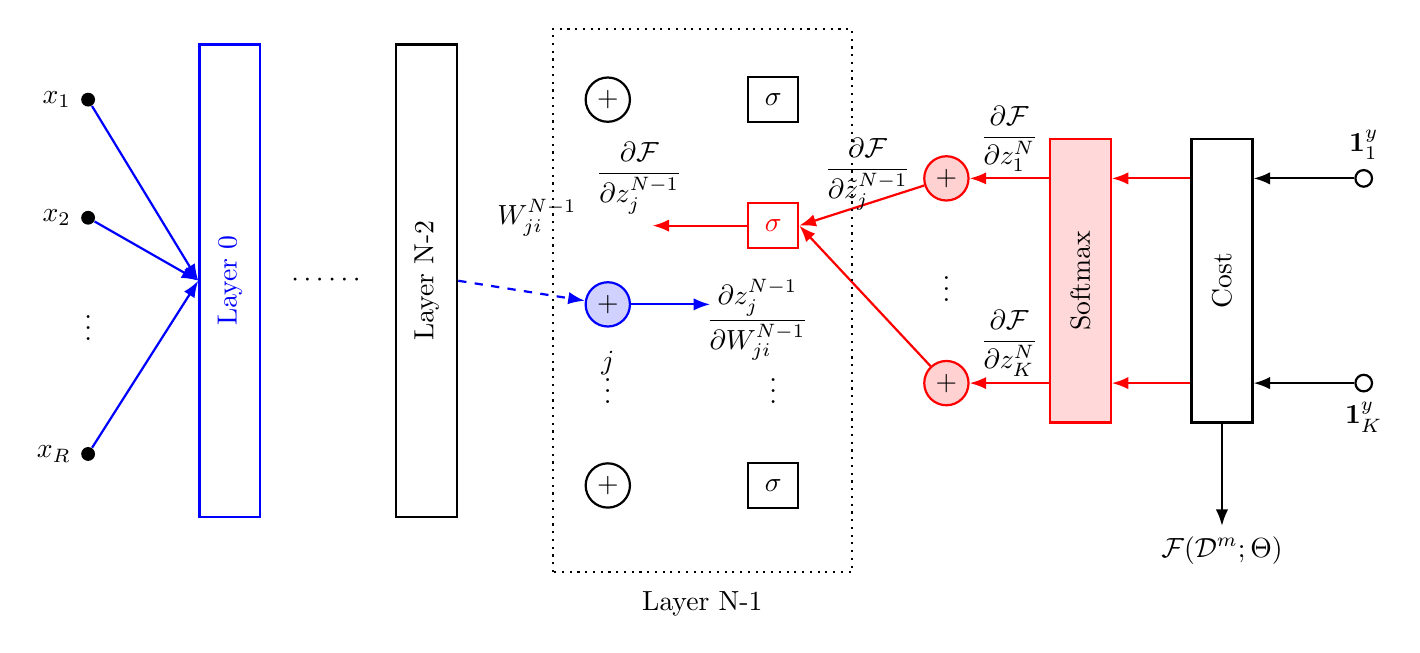
\begin{tikzpicture}[>=Latex]

    % ---- inputs (blue forward) ----
    \node[unit, label=left:{$x_1$}] (x1) at (0, 3)    {};
    \node[unit, label=left:{$x_2$}] (x2) at (0, 1.5)  {};
    \node                            (xd) at (0, 0.2)  {$\vdots$};
    \node[unit, label=left:{$x_R$}] (xR) at (0, -1.5) {};

    \node[opbox, minimum height=6cm, draw=fwdblue] (L0) at (1.8, 0.7)
        {\textcolor{fwdblue}{\vlabel{Layer 0}}};
    \node at (3.05, 0.7) {$\cdots\cdots$};
    \node[opbox, minimum height=6cm] (L2) at (4.3, 0.7) {\vlabel{Layer N-2}};

    \foreach \x in {x1,x2,xR}{ \draw[edge, fwdblue] (\x) -- (L0.west); }

    % ---- hidden layer N-1 : only middle unit active ----
    \node[sumop] (hA) at (6.6, 3)     {$+$};
    \node[sumop, draw=fwdblue, fill=fwdblue!18] (hB) at (6.6, 0.4) {$+$};
    \node        (hd) at (6.6, -0.6)  {$\vdots$};
    \node[sumop] (hC) at (6.6, -1.9)  {$+$};

    \node[opbox, minimum size=16pt] (gA) at (8.7, 3)     {$\sigma$};
    \node[opbox, minimum size=16pt, draw=bpred] (gB) at (8.7, 1.4)
        {\textcolor{bpred}{$\sigma$}};
    \node        (gd) at (8.7, -0.6)  {$\vdots$};
    \node[opbox, minimum size=16pt] (gC) at (8.7, -1.9)  {$\sigma$};

    % highlighted forward weight edge + derivative
    \draw[edge, fwdblue, dashed] (L2.east) -- (hB);
    \node at (5.7, 1.5) {$W_{ji}^{N-1}$};
    \node at (6.6, -0.35) {$j$};
    \draw[edge, fwdblue] (hB) -- ++(1.3, 0);
    \node at (8.5, 0.2) {$\dfrac{\partial z_j^{N-1}}{\partial W_{ji}^{N-1}}$};

    % ---- final linear layer (red backprop) ----
    \node[sumop, draw=bpred, fill=bpred!18] (fA) at (10.9, 2)    {$+$};
    \node        (fd) at (10.9, 0.7)  {$\vdots$};
    \node[sumop, draw=bpred, fill=bpred!18] (fB) at (10.9, -0.6) {$+$};

    % red backprop: final sums -> middle sigma (fan-in, leftward)
    \draw[edge, bpred] (fA) -- (gB.east);
    \draw[edge, bpred] (fB) -- (gB.east);

    % red backprop out of sigma (leftward)
    \draw[edge, bpred] (gB.west) -- ++(-1.2, 0);
    \node at (7.0, 2.0) {$\dfrac{\partial \mathcal{F}}{\partial z_j^{N-1}}$};
    \node at (9.9, 2.05) {$\dfrac{\partial \mathcal{F}}{\partial \tilde{z}_j^{N-1}}$};

    % ---- softmax / cost ----
    \node[opbox, minimum height=3.6cm, draw=bpred, fill=bpred!15]
        (soft) at (12.6, 0.7) {\vlabel{Softmax}};
    \node[opbox, minimum height=3.6cm] (cost) at (14.4, 0.7) {\vlabel{Cost}};

    % red backprop softmax -> final sums (leftward, exit the box's left edge)
    \draw[edge, bpred] (soft.west |- fA) -- (fA)
        node[wire, midway, above, black] {$\dfrac{\partial \mathcal{F}}{\partial z_1^N}$};
    \draw[edge, bpred] (soft.west |- fB) -- (fB)
        node[wire, midway, above, black] {$\dfrac{\partial \mathcal{F}}{\partial z_K^N}$};

    % red backprop cost -> softmax (leftward)
    \draw[edge, bpred] (cost.west |- fA) -- (soft.east |- fA);
    \draw[edge, bpred] (cost.west |- fB) -- (soft.east |- fB);

    % indicators (hollow, black, leftward into cost)
    \node[circle, draw, thick, fill=white, minimum size=6pt, inner sep=0pt,
          label=above:{$\mathbf{1}^y_1$}] (i1) at (16.2, 2)    {};
    \node[circle, draw, thick, fill=white, minimum size=6pt, inner sep=0pt,
          label=below:{$\mathbf{1}^y_K$}] (iK) at (16.2, -0.6) {};
    \draw[edge] (i1) -- (cost.east |- fA);
    \draw[edge] (iK) -- (cost.east |- fB);

    \draw[edge] (cost.south) -- ++(0, -1.3)
        node[below] {$\mathcal{F}(\mathcal{D}^m; \Theta)$};

    % dotted grouping box for layer N-1
    \draw[dotted, thick] (5.9, -3.0) rectangle (9.7, 3.9);
    \node at (7.8, -3.4) {Layer N-1};

\end{tikzpicture}
\end{document}
